\documentclass[aspectratio=169]{beamer}
%\documentclass[aspectratio=43]{beamer}

\usepackage{graphicx}  % Required for including images
\usepackage{natbib}
\usepackage{booktabs} % Top and bottom rules for tables
\usepackage{amssymb,amsthm,amsmath}
\usepackage{exscale}
\usepackage{natbib}
\usepackage{tikz}
\usepackage{listings}
\usepackage{color}
\usepackage{animate}
\usepackage{bm}
\usepackage{etoolbox}

% Setup TikZ
\usepackage{tikz}
\usetikzlibrary{arrows}
\tikzstyle{block}=[draw opacity=0.7,line width=1.4cm]
% Setup hyperref
\usepackage{hyperref}
\hypersetup{colorlinks=true}
\hypersetup{citecolor=porange}
\hypersetup{urlcolor=porange!80!}
\hypersetup{linkcolor=porange}

\newtheorem{proposition}{Proposition}
\newtheorem{remark}{Remark}
\newtheorem{principle}{Principle}

%% Writing quarters
\newcommand{\wQ}[1]{{\textcolor{white}{Q#1}}}
\newcommand{\bQ}[1]{{Q#1}}

% Uncomment appropriate command to disable/enable hiding
\newcommand{\mypause}{\pause}
%\newcommand{\mypause}{}
\newcommand{\myb}[1]{{\color{blue} {#1}}}

%% Commonly used macros
\newcommand{\eqr}[1]{Eq.\thinspace(#1)}
\newcommand{\pfrac}[2]{\frac{\partial #1}{\partial #2}}
\newcommand{\pfracc}[2]{\frac{\partial^2 #1}{\partial #2^2}}
\newcommand{\pfraca}[1]{\frac{\partial}{\partial #1}}
\newcommand{\pfracb}[2]{\partial #1/\partial #2}
\newcommand{\pfracbb}[2]{\partial^2 #1/\partial #2^2}
\newcommand{\spfrac}[2]{{\partial_{#1}} {#2}}
\newcommand{\mvec}[1]{\mathbf{#1}}
\newcommand{\gvec}[1]{\boldsymbol{#1}}
\newcommand{\script}[1]{\mathpzc{#1}}
\newcommand{\eep}{\mvec{e}_\phi}
\newcommand{\eer}{\mvec{e}_r}
\newcommand{\eez}{\mvec{e}_z}
\newcommand{\iprod}[2]{\langle{#1}\rangle_{#2}}

\DeclareMathAlphabet{\mathpzc}{OT1}{pzc}{m}{it}

%% Autoscaled figures
\newcommand{\incfig}{\centering\includegraphics}
\setkeys{Gin}{width=0.9\linewidth,keepaspectratio}

%Make the items smaller
\newcommand{\cramplist}{
	\setlength{\itemsep}{0in}
	\setlength{\partopsep}{0in}
	\setlength{\topsep}{0in}}
\newcommand{\cramp}{\setlength{\parskip}{.5\parskip}}
\newcommand{\zapspace}{\topsep=0pt\partopsep=0pt\itemsep=0pt\parskip=0pt}

\newcommand{\backupbegin}{
   \newcounter{finalframe}
   \setcounter{finalframe}{\value{framenumber}}
}
\newcommand{\backupend}{
   \setcounter{framenumber}{\value{finalframe}}
}

\usetheme[bullet=circle,% Use circles instead of squares for bullets.
          titleline=true,% Show a line below the frame title.
          ]{Princeton}

\title[{\tt }]{Flux-Limiters, Discontinuous Galerkin Schemes}%
\author[https://ast560.rtfd.io]%
{Ammar H. Hakim ({\tt ammar@princeton.edu}) \inst{1}}%

\institute[PPPL]
{ \inst{1} Princeton Plasma Physics Laboratory, Princeton, NJ %
}

\date[3/30/2021]{Princeton University, Course AST560, Spring 2021}

\begin{document}

\begin{frame}[plain]
  \titlepage
\end{frame}

\begin{frame}{Nonlinear flux limiters: Getting around Godunov's Theorem}
  \small%
  To get around Godunov's Theorem we need to construct a
  \emph{nonlinear scheme}, even for linear equations. One apporach is
  to use nonlinear flux-limiters:
  \begin{align*}
    \mvec{F}_{j+1/2} = \phi(r_{j+1}) \mvec{F}^H_{j+1/2} + \big(1-\phi(r_{j+1})\big) \mvec{F}^L_{j+1/2}
  \end{align*}
  where $\phi(r)>0$ is a \emph{limiter} function: chooses between
  \emph{high-order} and \emph{low-order} flux.
  \mypause%
  \begin{itemize} 
  \item What are the low- and high-order fluxes? For high-order
    fluxes: use either symmetric or higher-order upwind-biased
    recovery to construct the flux. For low-order use first-order
    upwind fluxes.
  \end{itemize}
  \mypause%
  The first-order upwind flux is ``Total-Variation Diminishing''
  (TVD), $\textrm{TV}(f^{n+1}) \le \textrm{TV}(f^n)$ where
  ``Total-Variation'' is defined as:
  \begin{align*}
    \textrm{TV}(f) = \sum_j | f_{j+1} - f_{j} |
  \end{align*}
\end{frame}

\begin{frame}{Nonlinear flux limiters}
  \small
  \begin{columns}
    \begin{column}{0.5\linewidth}
      The limiter function $\phi(r)$ depends on an estimate of the
      \emph{relative} slopes at an interface. For example, one choice
      is
      \begin{align*}
        r_{j+1/2} = \frac{\textrm{\textrm{slope at upwind-edge}}}{\textrm{slope at } j+1/2}
      \end{align*}
      (For systems of equations one needs limit each eigenvector
      instead). With this, choose a function that maintains TVD
      property. Eg, min-mod limiter
      \begin{align*}
        \phi(r) = \max\big(0, \min(2r, (1+r)/2,2) \big).
      \end{align*}
    \end{column}
    
    \begin{column}{0.5\linewidth}
      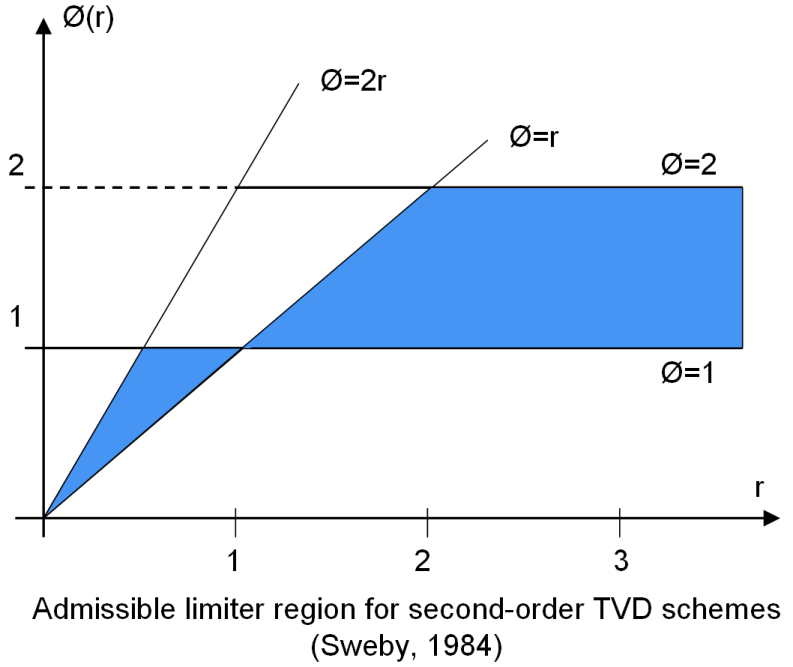
\includegraphics[width=\linewidth]{LimiterRegion.png}
    \end{column}
  \end{columns}
  See Wikipedia page
  \url{https://en.wikipedia.org/wiki/Flux_limiter}. (Not very
  high-quality but gives you a general idea).
\end{frame}

\begin{frame}{Nonlinear flux limiters: No ``Perfect'' Limiter!}
  \small
  \begin{columns}
    \begin{column}{0.5\linewidth}
      \begin{itemize}
      \item Unfortunately, there is no perfect limiter (though some
        come close to perfection): depends on problem and best to
        implement many!
      \item Most limiters ``chop off'' genuine maxima/minima: notice
        that $\phi(r<0) = 0$ which means that if there is a genuine
        maxima/minima then low-order flux is selected.
      \item Tricky to distinguish step-function from parabola!
        ``Best'' limiter (IMO): Suresh and Huynh, JCP {\bf 136}, 83-99
        (1997). Not an easy paper to understand.
      \end{itemize}
    \end{column}
    
    \begin{column}{0.5\linewidth}
      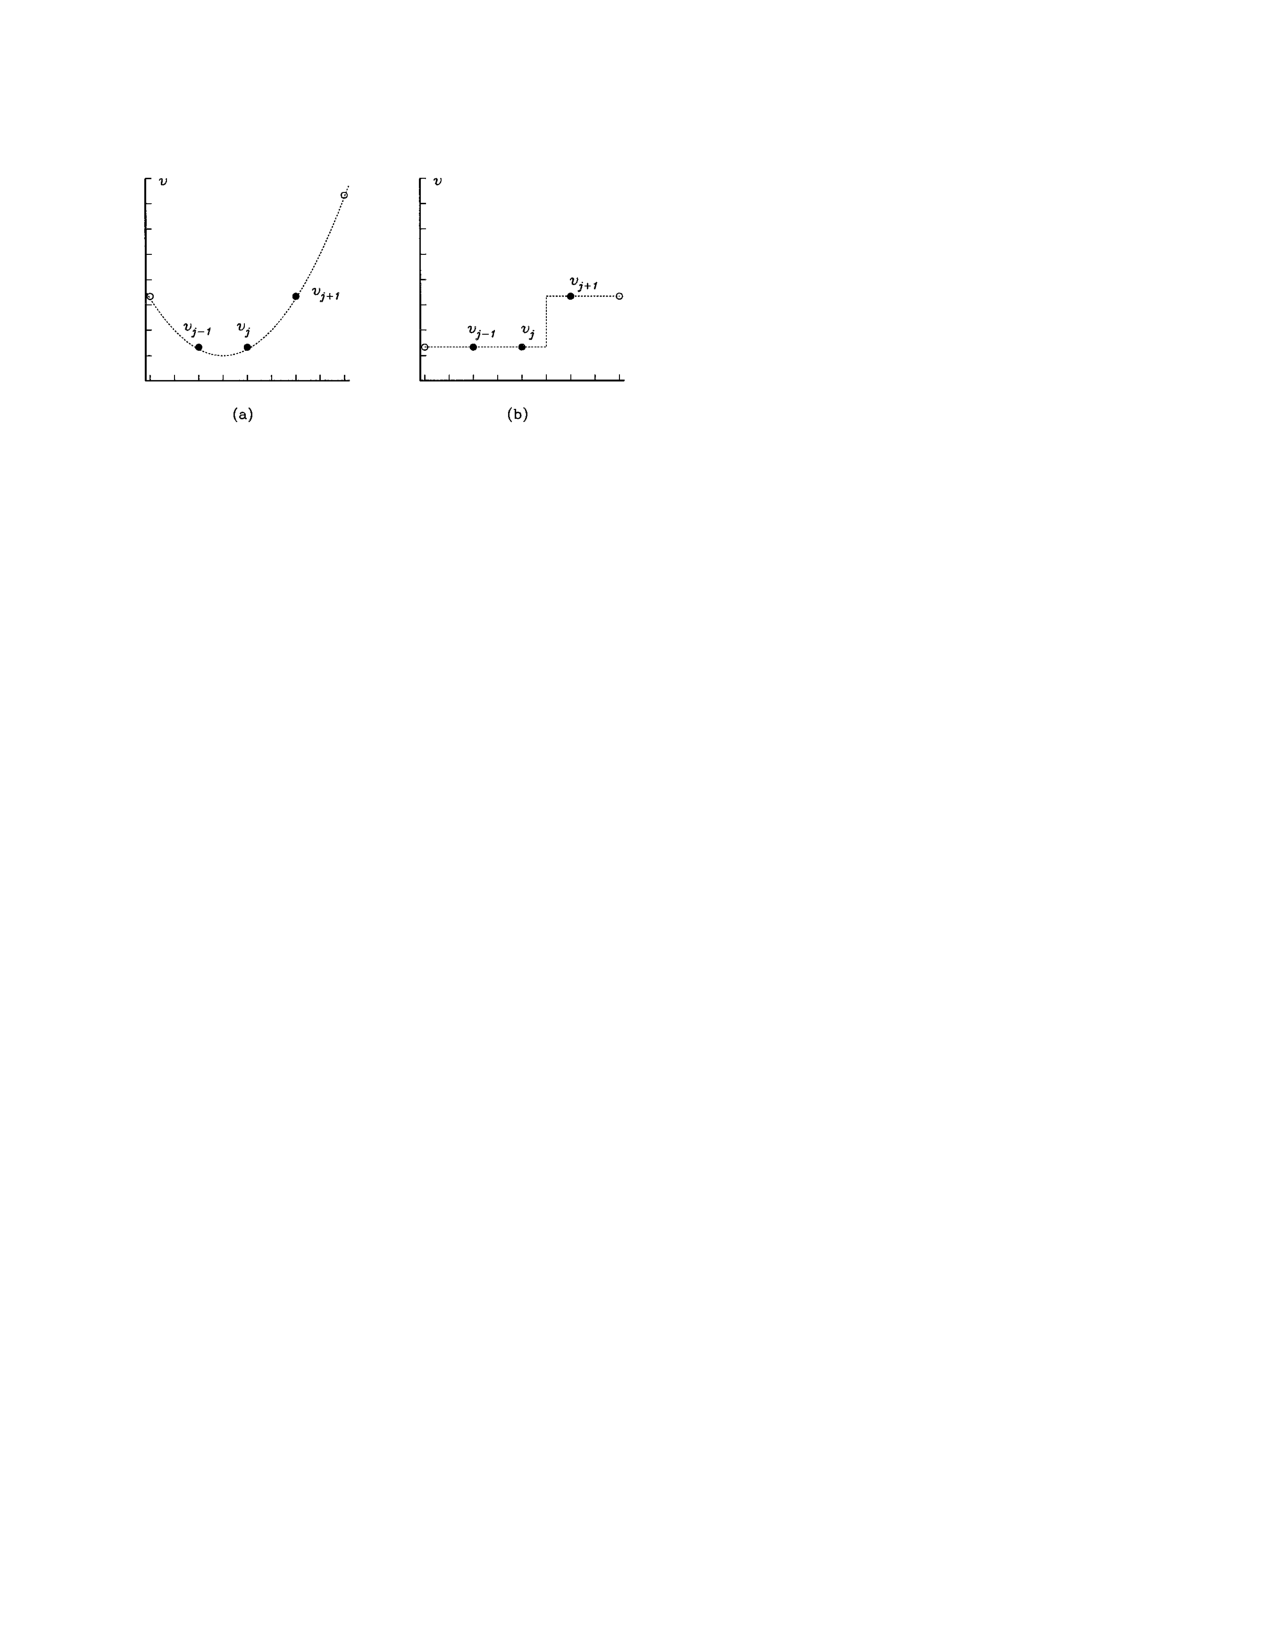
\includegraphics[width=\linewidth]{suresh-huynh.pdf}
    \end{column}
  \end{columns}
\end{frame}  

\begin{frame}{Generalizing recovery: path to discontinous Galerkin schemes}
  \begin{itemize}
  \item In FV scheme we used \emph{cell-averages} to recover interface
    values for use in numerical fluxes%
    \mypause%
  \item What if we store more than just cell-averages? One can imagine
    in addition, mean-slope, mean-quadratic moments. Lead naturally to
    the concept of discontinous Galerkin schemes.
  \end{itemize}
  \mypause%
  The key connection is the concept of \emph{weak-equality}. Consider
  an interval $I$ and select a finite-dimensional function space on
  it, spanned by set of basis functions $\{ \psi_k \}$,
  $k=1,\ldots,N$. Choose an inner product, for example
  \begin{align*}
    (f, g) \equiv \int_I f(x) g(x) \thinspace dx.
  \end{align*}  
\end{frame}

\begin{frame}{Weak-equality}
  \small
  \begin{definition}[Weak equality]
    Two functions, $f$ and $g$ are said to be \emph{weakly equal} if
    \begin{align*}
      (\psi_k,f-g) = 0
    \end{align*}
    for all $k=1,\ldots,N$. We denote weak equality by
    \begin{align*}
      f \doteq g.
    \end{align*}
  \end{definition}  
  \begin{itemize}
  \item When we recovered polynomials across an interface in FV scheme
    we effectively choose a function space, $\{1 \}$ , with only
    \emph{one} basis function!
  \item In DG we can choose as many as we like: allows significant
    flexibility in designing accurate and compact schemes; suprisingly
    accurate for some problems.
  \end{itemize}
\end{frame}

% ----------------------------------------------------------------
\begin{frame}{What are discontinuous Galerkin schemes?}

  \begin{block}{}
    Discontinuous Galerkin schemes are a class of \emph{Galerkin}
    schemes in which the solution is represented using \emph{piecewise
      discontinuous} functions.
  \end{block}
  \mypause
  \begin{itemize}
    \item \emph{Galerkin} minimization
    \item Piecewise \emph{discontinuous} representation
  \end{itemize}
  \mypause
  Goal of this lecture is to understand conceptual meaning of
  discontinuous Galerkin schemes and understand how to use them to
  solve PDEs. Much is left out as the literature on DG is vast, but
  will aim to cover key conceptual ideas. Outline

  \begin{itemize}
  \item Discontinuous Galerkin representation, recovery and
    weak-equalities
  \item DG scheme for linear advection and extension to Maxwell
    equations. Aspects of DG for nonlinear problems
  \item Application of DG to plasma kinetic equations
  \end{itemize}  
  
\end{frame}  

\begin{frame}{DG represent state-of-art for solution of PDEs}

  DG algorithms hot topic in CFD and applied mathematics.
  \begin{itemize}
    \small
  \item First introduced by Reed and Hill in 1973 as a conference
    paper to solve steady-state neutron transport equations. More than
    2100 citations. \mypause
  \item Some earlier work on solving \emph{elliptic} equations by
    Nitsche in 1971 (original paper in German). Introduced the idea of
    ``interior penalty''. Usually, though, DG is not used for elliptic
    problems. Paradoxically, perhaps DG may be even better for certain
    elliptic/parabolic problems. \mypause
  \item Key paper for nonlinear systems in multiple dimensions is by
    Cockburn and Shu (JCP, {\bf 141}, 199-224, 1998). More than 1700
    citations. \mypause
  \item Almost continuous stream of papers in DG, both for fundamental
    formulations and applications to physics and engineering
    problems. This continues to be an active area of research, and at
    present \emph{DG is under-utilized in plasma physics}.
  \end{itemize}

\end{frame}
% ----------------------------------------------------------------

% ----------------------------------------------------------------
\begin{frame}{Essential idea of Galerkin methods: $L_2$ minimization
    of errors}
  \small%
  There two key ingredients in a Galerkin scheme: selection of a
  finite-dimensional space of functions and a definition of errors.
  \mypause%

  \begin{itemize}\small
  \item Consider a interval $[-1,1]$. On this, we can choose Legendre
    polynomials $P_l(x)$ up to some order $l<N$ as a \emph{basis-set}.
  \item We need to \emph{define} a way to measure errors on this
    function space. One way to do this is to select an inner product
    and then use it to define a norm. For example consider the
    inner-product
    \begin{align*}
      (f,g) = \int_{-1}^1 f(x) g(x) \thinspace dx
    \end{align*}
    using which we can define the $L_2$ norm
    \begin{align*}
      \| f \|_2 = (f, f)
    \end{align*}
  \end{itemize}
  Once we have selected the finite-dimensional space of functions and
  a norm, we can use it to construct a Galerkin method.
  
\end{frame}
% ----------------------------------------------------------------  

% ----------------------------------------------------------------  

% ----------------------------------------------------------------
\begin{frame}{Essential idea of Galerkin methods: $L_2$ minimization
    of errors}
  \small
  Consider a general time-dependent problem on $x\in [-1,1]$:
  \begin{align*}
    f'(x,t) = G[f]
  \end{align*}
  where $G[f]$ is some operator. To approximate it expand $f(x)$ with
  our basis functions $P_k(x)$,
  \begin{align*}
    f(x,t) \approx f_h(x,t)  = \sum_{k=1}^N f_k(t) P_k(x)
  \end{align*}
  This gives discrete system
  \begin{align*}
    \sum_{k=1}^N f_k' P_k(x) = G[f_h]
  \end{align*}
  \mypause
  \begin{block}{Question}
    How to determine $f_k'$ in an optimum manner?
  \end{block}
  
\end{frame}
% ----------------------------------------------------------------

% ----------------------------------------------------------------
\begin{frame}{Essential idea of Galerkin methods: $L_2$ minimization
    of errors}
  \small
  Answer: Do an $L_2$ minimization of the error, i.e. find $f_k'$ such
  that the error as \emph{defined by our selected norm} is minimized.
  \begin{align*}
    E_N = \left \| \sum_{k=1}^N f_k' P_k(x) - G[f_h] \right \|_2
    = 
    \int_{-1}^1 \left[
      \sum_{k=1}^N f_k' P_k(x) - G[f_h]\right]^2\thinspace dx
  \end{align*}
  For minimum error $\partial E_N/\partial f_m' = 0$ for all
  $k=1,\ldots,N$. This leads to the linear system that determines the
  coefficients $f_k'$
  \begin{align*}
    \int_{-1}^1 P_m(x) \left(
      \sum_{k=1}^N f_k' P_k(x) - G[f_h]
    \right)\thinspace dx = 0
  \end{align*}
  for all $m=1,\ldots,N$. This will give
  \begin{align*}
    f_k'  = \frac{2k+1}{2}\int_{-1}^1 P_k(x) G[f_h] \thinspace dx
  \end{align*}  
\end{frame}
% ----------------------------------------------------------------

% ----------------------------------------------------------------
\begin{frame}{Typical $L_2$ fit look like for Galerkin scheme?}
  Consider finding the best-fit on finite-dimensional space for the
  function $f(x) = 3+(x-0.5)^4 + 2x^3 - 5x^2$ on $x\in[-1,1]$. Choose
  \emph{normalized} Legendre polynomials as basis functions.
  \begin{figure}
    \setkeys{Gin}{width=0.25\linewidth,keepaspectratio}
    \incfig{fit-p0.pdf}
    \incfig{fit-p1.pdf}
    \incfig{fit-p2.pdf}
    \incfig{fit-p4.pdf}
    \caption{Best $L_2$ fit with $p=0$, $p=1$, $p=2$ and $p=4$ for
      $f(x) = 3+(x-0.5)^4 + 2x^3 - 5x^2$ on $x\in[-1,1]$.}
  \end{figure}

\end{frame}
% ----------------------------------------------------------------

\begin{frame}{Typical $L_2$ fit look like: \emph{discontinuous}
    Galerkin scheme}
  In discontinuous Galerkin schemes we split interval into cells and
  use Galerkin scheme in each cell. This will naturally lead to
  \emph{discontinuities} across cell boundaries.
  \begin{figure}
    \setkeys{Gin}{width=0.5\linewidth,keepaspectratio}
    \incfig{v1m1.png}
    \incfig{v2m1.png}
    \caption{The best $L_2$ fit of $x^4+\sin(5x)$ with piecewise
      linear (left) and quadratic (right) basis functions.}
  \end{figure}

\end{frame}
% ----------------------------------------------------------------

\begin{frame}{Weak-equality and recovery}
  \footnotesize
  \begin{itemize}\cramplist
  \item It is important to remember that the discontinuous Galerkin
    solution is a \emph{representation} of the solution and not the
    solution itself.
  \item Notice that even a continuous function will, in general, have
    a discontinuous \emph{representation} in DG.
  \end{itemize}
  \mypause%
  We can formalize this idea using the concept of
  \emph{weak-equality}.

  \begin{definition}[Weak equality]
    Two functions, $f$ and $g$ are said to be \emph{weakly equal} if
    \begin{align*}
      (\psi_k,f-g) = 0
    \end{align*}
    for all $k=1,\ldots,N$. We denote weak equality by
    \begin{align*}
      f \doteq g.
    \end{align*}
  \end{definition}  
  
\end{frame}

% ----------------------------------------------------------------  

\begin{frame}{Weak-equality and recovery}
  \footnotesize
  \begin{itemize}
  \item Notice that weak-equality depends on the function space as
    well as the inner-product we selected.
  \item The Galerkin $L_2$ minimization is equivalent to, for example,
    restating that
    \begin{align*}
      f'(x,t) \doteq G[f]
    \end{align*}
    This implies
    \begin{align*}
      \left(\psi_k, f'(x,t)- G[f] \right) = 0
    \end{align*}
    which is exactly what we obtained by minimizing the error defined    
    using the  $L_2$ norm. \mypause
  \item Hence, we can say that the \emph{DG scheme only determines the
      solution in the weak-sense}, that is, all functions that are
    weakly equal to DG representation can be potentially interpreted
    as the actual solution.
  \item This allows a powerful way to construct schemes with desirable
    properties by \emph{recovering} weakly-equal functions using the
    DG representations.
  \end{itemize}

\end{frame}

% ----------------------------------------------------------------  
\begin{frame}{Example of recovery: Exponential recovery in a cell}

  \begin{itemize}
  \item Consider we have a linear representation of the particle
    distribution function $f_h(x) = f_0 + x f_1$ in a cell.
  \item We can use this to \emph{reconstruct} an exponential function
    that has the desirable property that it is \emph{positive}
    everywhere in the cell. That is, we want to find
    \begin{align*}
      \exp(g_0 + g_1 x) \doteq f_0 + x f_1
    \end{align*}
  \item This will lead to a coupled set of nonlinear equations to
    determine $g_0$ and $g_1$
  \item Note that this process is not always possible: we need $f_0>0$
    as well as the condition $|f_1| \le 3 f_0$. Otherwise, the $f_h$
    is not realizable (i.e. there is no positive distribution function
    with the same moments as $f_h$).
  \end{itemize}
\end{frame}

% ----------------------------------------------------------------

\begin{frame}{Example of recovery: Exponential recovery in a cell}
  \begin{figure}
    \setkeys{Gin}{width=0.5\linewidth,keepaspectratio}
    \incfig{exp-fit-1.png}
    \incfig{exp-fit-2.png}
    \caption{Recovery of exponential function (black) from linear
      function (red). Left plot is for $f_0 = 1$, $f_1 = 1$ and right
      for $f_0 = 1$ and $f_1 = 2$.}
  \end{figure}  
\end{frame}

% ----------------------------------------------------------------

\begin{frame}{Discontinuous Galerkin scheme for linear advection}
  Consider the 1D passive advection equation on $I\in [L,R]$
  \begin{align*}
    \pfrac{f}{t} + \lambda \pfrac{f}{x} = 0
  \end{align*}
  with $\lambda$ the constant advection speed. $f(x,t) = f_0(x-\lambda
  t)$ is the exact solution, where $f_0(x)$ is the initial
  condition. Designing a good scheme is much harder than it looks.
  \mypause
  \begin{itemize}
  \item Discretize the domain into elements $I_j\in
    [x_{j-1/2},x_{j+1/2}]$
  \item Pick a finite-dimensional function space to represent the
    solution. For DG we usually pick polynomials in each cell but
    allow discontinuities across cell boundaries
  \item Expand $f(x,t) \approx f_h(x,t) = \sum_k f_k(t) w_k(x)$.
  \end{itemize}  
\end{frame}

% ----------------------------------------------------------------
\begin{frame}{Find the coefficients that minimize the $L_2$ norm of
    the residual}

  The discrete problem in DG is stated as: find $f_h$ in the function
  space such that for each basis function $\varphi$ we have
  \begin{align*}
    \int_{I_j} \varphi\left(
      \pfrac{f_h}{t} 
      + \lambda \pfrac{f_h}{x}
      \right)
    \thinspace dx = 0.
  \end{align*}
  Integrating by parts leads to the discrete \emph{weak-form}
  \begin{align*}
    \int_{I_j} \varphi \pfrac{f_h}{t}\thinspace dx
    +
    \lambda \varphi_{j+1/2}\hat{F}_{j+1/2} - \lambda \varphi_{j-1/2}\hat{F}_{j-1/2}
    -
    \int_{I_j}  \frac{d\varphi}{dx}\lambda f_h\thinspace dx = 0.
  \end{align*}
  Here $\hat{F}_{} = \hat{F}(f^+_h,f^-_h)$ is the consistent
  \emph{numerical flux} on the cell boundary. Integrals are performed
  using high-order quadrature schemes.
  
\end{frame}
% ----------------------------------------------------------------

% ----------------------------------------------------------------
\begin{frame}{Need to select numerical flux}

  \begin{columns}
    \begin{column}{0.5\textwidth}
      \begin{itemize}
        \small
      \item Take averages (central fluxes)
        \begin{align*}
          \hat{F}(f^+_h,f^-_h) = \frac{1}{2}(f_h^+ + f_h^-)
        \end{align*}
      \item Use upwinding (upwind fluxes)
        \begin{align*}
          \hat{F}(f^+_h,f^-_h) &= f_h^- \quad\mathrm{\lambda>0} \\
          &= f_h^+ \quad\mathrm{\lambda<0}
        \end{align*}
      \end{itemize}
    \end{column}
    \begin{column}{0.55\textwidth}
      \begin{figure}
        \setkeys{Gin}{width=1.0\linewidth,keepaspectratio}
        \incfig{v1m1-anno.png}
      \end{figure}
    \end{column}
  \end{columns}

\end{frame}
% ----------------------------------------------------------------

% ----------------------------------------------------------------
\begin{frame}{Example: Piecewise constant basis functions}
  
  \begin{itemize}
  \item A central flux with piecewise constant basis functions leads
    to the familiar central difference scheme
    \begin{align*}
      \pfrac{f_{j}}{t} + \lambda\frac{f_{j+1}-f_{j-1}}{2\Delta x} = 0
    \end{align*}
  \item An upwind flux with piecewise constant basis functions leads
    to the familiar upwind difference scheme (for $\lambda>0$)
    \begin{align*}
      \pfrac{f_{j}}{t} + \lambda \frac{f_{j}-f_{j-1}}{\Delta x} = 0
    \end{align*}
  \end{itemize}
  Solution is advanced in time using a suitable ODE solver, usually
  strong-stability preserving Runge-Kutta methods. (See G2 website)
\end{frame}
% ----------------------------------------------------------------

% ----------------------------------------------------------------
\begin{frame}{Example: Piecewise constant basis functions with central
    flux}

  \begin{figure}
    \setkeys{Gin}{width=0.6\linewidth,keepaspectratio}
    \incfig{advection-p0-c.png}
    \caption{Advection equation solution (black) compared to exact
      solution (red) with central fluxes and piecewise constant basis
      functions.}
  \end{figure}

\end{frame}
% ----------------------------------------------------------------

% ----------------------------------------------------------------
\begin{frame}{Example: Piecewise constant basis functions
    with upwind flux}

  \begin{figure}
    \setkeys{Gin}{width=0.6\linewidth,keepaspectratio}
    \incfig{advection-p0.png}
    \caption{Advection equation solution (black) compared to exact
      solution (red) with upwind fluxes and piecewise constant basis
      functions.}
  \end{figure}

\end{frame}
% ----------------------------------------------------------------

\begin{frame}{Passive advection with piecewise linear basis functions}
  \small%
  To get better results, we can use piecewise linear polynomials
  instead. That is, select the basis functions
  \begin{align*}
    \varphi \in \{1, 2(x-x_j)/\Delta x\}
  \end{align*}
  In terms of which the solution in each cell is expanded as
  $f_j(x,t) = f_{j,0} + 2f_{j,1}(x-x_j)/\Delta x$. With this, some
  algebra shows that we have the update formulas for \emph{each stage}
  of a Runge-Kutta method
  \begin{align*}
    f^{n+1}_{j,0} &=
                    f_{j,0}^n
                    - \sigma
                    \left(\hat{F}_{j+1/2}-\hat{F}_{j-1/2} \right)
                    \\
    f^{n+1}_{j,1} &=
                    f_{j,1}^n
                    - 3\sigma
                    \left(
                    \hat{F}_{j+1/2}+\hat{F}_{j-1/2}
                    \right)
                    + 6\sigma f_{j,0}    
  \end{align*}
  where $\sigma \equiv \lambda\Delta t/\Delta x$. As these are explicit
  schemes we need to ensure time-step is sufficiently small. Usually,
  we need to ensure $\sigma = \lambda \Delta t/\Delta x \le 1/(2p+1)$.
\end{frame}

% ----------------------------------------------------------------

% ----------------------------------------------------------------
\begin{frame}{Passive advection with piecewise linear basis functions}

  \begin{figure}
    \setkeys{Gin}{width=0.5\linewidth,keepaspectratio}
    \incfig{advection-p1.png}
    \caption{Advection equation solution (black) compared to exact
      solution (red) with upwind fluxes and piecewise linear basis
      functions.}
  \end{figure}
  In general, with upwind fluxes and linear basis functions numerical
  diffusion goes like $|\lambda| \Delta x^3 \partial^4 f/ \partial
  x^4$.
\end{frame}
% ----------------------------------------------------------------

\begin{frame}{Properties of the discrete equations}
  From the continuous passive advection equation we can show that, on
  a periodic domain the total particles are conserved
  \begin{align*}
    \frac{d}{dt}\int_I f \thinspace dx = 0
  \end{align*}
  Also, the $L_2$ norm of the solution is also conserved
  \begin{align*}
    \frac{d}{dt}\int_I \frac{1}{2} f^2 \thinspace dx = 0
  \end{align*}  

  We would like to know if our discrete scheme \emph{inherits or
    mimics these properties}. Sometimes, methods in which the discrete
  scheme inhert important properties from the continuous equations are
  called \emph{mimetic} methods. However, note that in general it is
  impossible to inhert \emph{all} properties and often it is not
  desirable to do so.
  
\end{frame}

% ----------------------------------------------------------------

\begin{frame}{To prove properties start from discrete weak-form}
  \footnotesize
  To understand properties of the scheme we must (obviously) use the
  \emph{discrete weak-form} as the starting point.
  \begin{align*}
    \int_{I_j} \varphi \pfrac{f_h}{t}\thinspace dx
    +
    \lambda \varphi_{j+1/2}\hat{F}_{j+1/2} - \lambda \varphi_{j-1/2}\hat{F}_{j-1/2}
    -
    \int_{I_j}  \frac{d\varphi}{dx}\lambda f_h\thinspace dx = 0.
  \end{align*}
  A general technique is to use a function belonging to the
  \emph{finite-dimensional function space} as the test function
  $\varphi$ in the discrete weak-form.
  \mypause%

  Example: consider we set $\varphi = 1$. Then we get
  \begin{align*}
    \sum_j \int_{I_j} \pfrac{f_h}{t}\thinspace dx
    +
    \lambda \sum_j \left(
    \hat{F}_{j+1/2} - \hat{F}_{j-1/2}
    \right) = 0.
  \end{align*}
  The second term sums to zero and so we have shown that
  \begin{align*}
    \frac{d}{dt}\sum_j \int_{I_j} f_h\thinspace dx = 0.
  \end{align*}  
\end{frame}

\begin{frame}{To prove properties start from discrete weak-form}
  \footnotesize%
  Now, consider we use the \emph{solution itself} as the test
  function. We can do this as the solution, by definition, belongs to
  the finite-dimensional function space. We get
  \begin{align*}
    \sum_j \int_{I_j} f_h \pfrac{f_h}{t}\thinspace dx
    +
    \sum_j \left(f_{hj+1/2}^-\hat{F}_{j+1/2} - f_{hj-1/2}^+\hat{F}_{j-1/2}\right)
    -
    \sum_j \int_{I_j}  \frac{d f_h}{dx} f_h\thinspace dx = 0
  \end{align*}
  We can write the last term as
  \begin{align*}
    \sum_j \int_{I_j}  \frac{1}{2} \frac{d}{dx} f_h^2 \thinspace dx
    = \frac{1}{2} \sum_j \left[ \left(f_{hj+1/2}^-\right)^2  - \left(f_{hj-1/2}^+\right)^2 \right]
  \end{align*}
  If we use \emph{upwind fluxes} we can show that we get
  \begin{align*}
    \frac{d}{dt} \sum_j \int_{I_j}  f_h^2 \thinspace dx
    =
    -\sum_j \left(f_{hj+1/2}^- - f_{hj-1/2}^+\right)^2 \le 0.
  \end{align*}
  Hence, the $L_2$ norm of the solution \emph{will decay and not
    remain constant}. However, this is the desirable behavior as it
  ensures $L_2$ stability of the discrete system. With central fluxes
  the $L_2$ norm is conserved. (Prove this)
\end{frame}

% ----------------------------------------------------------------

\begin{frame}{Summary of DG schemes for passive advection equation}

  \begin{itemize}
  \item Pick basis functions. These are usually piecewise polynomials,
    but could be other suitable functions.
  \item Construct discrete weak-form using integration by parts.
  \item Pick suitable numerical fluxes for the surface integrals.
  \item Use Runge-Kutta (or other suitable) schemes for evolving the
    equations in time.
  \item To prove properties of the scheme, start from the discrete
    weak-form and use appropriate test-functions and simplify.
  \end{itemize}

\end{frame}
% ----------------------------------------------------------------

\begin{frame}{How to discretize parabolic equations with DG?}
  \footnotesize%
  \begin{itemize}
  \item DG is traditionally used to solve hyperbolic PDEs. However, DG is
    also very good for the solution of parabolic PDEs.
  \item One challenge here is that parabolic PDEs have \emph{second}
    derivatives and it is not clear at first how a discontinuous
    representation can allow solving such systems.
  \end{itemize}
  Consider the diffusion equation (subscripts represent derivatives)
  \begin{align*}
    f_t = f_{xx}
  \end{align*}
  Choose function space and multiply by test function in this space to
  get weak form
  \begin{align*}
    \int_{I_j} \varphi f_t \thinspace dx =   \varphi f_x \bigg|^{x_{j+1/2}}_{x_{j-1/2}}
    -
    \int_{I_j} \varphi_{x} f_x \thinspace dx.
  \end{align*}
  In DG, as $f$ is discontinuous, it is not clear how to compute the
  derivative across the discontinuity at the cell interface in the
  first term. (See SimJ JE16).
  
\end{frame}

% ----------------------------------------------------------------

\begin{frame}{Lets revisit weak-equality and recovery}
  \begin{definition}[Weak equality]
    Two functions, $f$ and $g$ are said to be \emph{weakly equal} if
    \begin{align*}
      (\psi_k,f-g) = 0
    \end{align*}
    for all $k=1,\ldots,N$. We denote weak equality by
    \begin{align*}
      f \doteq g.
    \end{align*}
  \end{definition}
  Recall that the DG solution is only a \emph{representation} of the
  solution and not the solution itself. Hence, we can consider the
  following ``inverse'' problem: given a discontinuous solution across
  two cells, is it possible to \emph{recover} a \emph{continuous
    representation} that can then be used in the above weak-form?
\end{frame}

% ----------------------------------------------------------------

\begin{frame}{Use weak-equality to \emph{recover} continuous function}
  \begin{figure}%
    \setkeys{Gin}{width=0.5\linewidth,keepaspectratio}
    \incfig{v1m1-2c.png}
    \caption{Given piecewise linear representation (black) we want to
      recover the continuous function (red) such that {\bf moments of
        recovered and linear representation are the same in the
        respective cells}. }
  \end{figure}
\end{frame}

% ----------------------------------------------------------------

\begin{frame}{Use weak-equality to \emph{recover} continuous function}

  \footnotesize
  \begin{itemize}
  \item Consider recovering $\hat{f}$ on the interval $I=[-1,1]$, from a
    function, $f$, which has a single discontinuity at $x=0$.
  \item Choose some function spaces $\mathcal{P}_L$ and
    $\mathcal{P}_R$ on the interval $I_L = [-1,0]$ and $I_R = [0,1]$
    respectively.
  \item Reconstruct a continuous function $\hat{f}$ such that
    \begin{align*}
      \hat{f} &\doteq f_L \quad x \in I_L \quad\mathrm{on}\
                \mathcal{P}_L \\
      \hat{f} &\doteq f_R \quad x \in I_R \quad\mathrm{on}\ \mathcal{P}_R.
    \end{align*}
    where $f = f_L$ for $x\in I_L$ and $f = f_R$ for $x\in I_R$.
  \item To determine $\hat{f}$, use the fact that given $2N$ pieces of
    information, where $N$ is the number of basis functions in
    $\mathcal{P}_{L,R}$, we can construct a polynomial of maximum
    order $2N-1$. We can hence write
    \begin{align*}
      \hat{f}(x) = \sum_{m=0}^{2N-1} \hat{f}_m x^m.
    \end{align*}
    Plugging this into the weak-equality relations gives a
    \emph{linear} system for $\hat{f}_m$.
  \end{itemize}
\end{frame}

% ----------------------------------------------------------------
\begin{frame}{Use recovered function in weak-form}
  Once we have determined $\hat{f}$ we can use this in the discrete
  weak-form of the diffusion equation:
  \begin{align*}
    \int_{I_j} \varphi f_t \thinspace dx =   \varphi \hat{f}_x \bigg|^{x_{j+1/2}}_{x_{j-1/2}}
    -
    \int_{I_j} \varphi_{x} f_x \thinspace dx.
  \end{align*}
  Note that now as $\hat{f}$ is continuous at the cell interface there
  is no issue in computing its derivative. We can, in fact, do a
  second integration by parts to get another discrete weak-form
  \begin{align*}
    \int_{I_j} \varphi f_t \thinspace dx =   (\varphi \hat{f}_x - \varphi_x \hat{f})\bigg|^{x_{j+1/2}}_{x_{j-1/2}}
    +
    \int_{I_j} \varphi_{xx} f \thinspace dx.
  \end{align*}
  This weak-form has certain advantages as the second term does not
  contain derivatives (which may be discontinuous at cell
  boundary).
\end{frame}

\end{document}


\begin{frame}{}
\end{frame}

\begin{columns}
  
  \begin{column}{0.6\linewidth}
  \end{column}
  
  \begin{column}{0.4\linewidth}
    \includegraphics[width=\linewidth]{fig/Kinsey_2011_Pfus_vs_T.pdf}
  \end{column}
\end{columns}

% ----------------------------------------------------------------
